\begin{frame}{Konstrukcija pravokotnice}
	\centering
	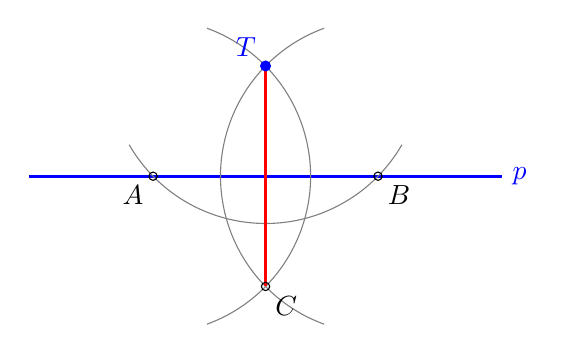
\begin{tikzpicture}
		\coordinate (T) at (0, 1.4);
		\draw[blue, very thick] (-3, 0) -- (3, 0) node[right] {$p$};
		\draw[gray] (T) ++(210:2) arc (210:330:2);
		\coordinate (A) at (-1.4282857, 0);
		\coordinate (B) at (1.4282857, 0);
		\draw[gray] (A) ++(-70:2) arc (-70:70:2);
		\draw[gray] (B) ++(250:2) arc (250:110:2);
		\coordinate (C) at (0, -1.4);
		\draw[red, very thick] (T) -- (C);
		\fill[blue] (T) circle (2pt) node[above left] {$T$};
		\draw (A) circle (1.5pt) node[below left] {$A$};
		\draw (B) circle (1.5pt) node[below right] {$B$};
		\draw (C) circle (1.5pt) node[below right] {$C$};
	\end{tikzpicture}
\end{frame}
